\documentclass[tikz, border=3mm]{standalone}
\usepackage{tikz}
\usetikzlibrary{arrows.meta, calc} % calc library for midpoints

\begin{document}
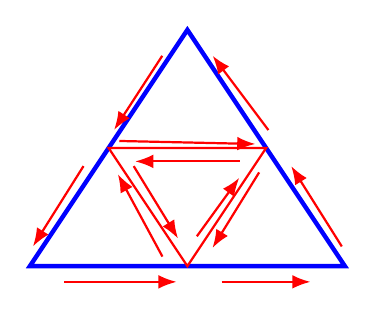
\begin{tikzpicture}[
    >=Latex, % Set default arrow tip style
    arrowstyle/.style={->, red, thick, shorten <=1pt, shorten >=1pt} % Style for arrows
]

    % Define Outer Triangle Vertices (adjust size/shape if needed)
    % Using a slightly shorter height for better visual spacing
    \coordinate (A) at (-2, 0);
    \coordinate (B) at (2, 0);
    \coordinate (C) at (0, 3);

    % Define Inner Triangle Vertices (midpoints of outer sides)
    \coordinate (D) at ($(A)!0.5!(B)$); % Midpoint of AB -> (0, 0)
    \coordinate (E) at ($(B)!0.5!(C)$); % Midpoint of BC -> (1, 1.5)
    \coordinate (F) at ($(C)!0.5!(A)$); % Midpoint of CA -> (-1, 1.5)
    
    
%    ############# OUTSIDE TRIANGLES
    \coordinate (LA1) at ($(C)+(-0.3,-0.3)$);
    \coordinate (LA2) at ($(F) +(0.05,0.2)$);
    \coordinate (LB1) at ($(F) + (-0.3, -0.2)$);
    \coordinate (LB2) at ($(A)+(0.02,0.22)$);
\coordinate (RA1) at ($(C)+(0.3,-0.3)$);
 \coordinate (RA2) at ($(E) +(0.05,0.2)$);
    \coordinate (RB1) at ($(E) + (0.3, -0.2)$);
    \coordinate (RB2) at ($(B)+(-0.02,0.22)$);
    \coordinate (DA1) at ($(A)+(0.4,-0.2)$);
    \coordinate (DB1) at ($(D)+(0.4,-0.2)$);
    \coordinate (DB2) at ($(B)+(-0.4,-0.2)$);
    \coordinate (DA2) at ($(D)+(-0.1, -0.2)$);
    
    
%    ######## for RED TRIANGLE
    \coordinate (red_UP1) at ($(F)+(0.1,0.09)$);
    \coordinate (red_LEFT1) at ($(F)+(0.1,-0.3)$);
    \coordinate (red_RIGHT1) at ($(D)+(0.3,0.2)$);
  	    \coordinate (red_UP2) at ($(E)+(-0.1,0.05)$);
    \coordinate (red_LEFT2) at ($(D)+(-0.3,0.09)$);
    \coordinate (red_RIGHT2) at ($(E)+(-0.07,-0.28)$);

%############# for inside of inner triangle
 \coordinate (inside_UP1) at ($(E)+(-0.3,-0.17)$);
\coordinate (inside_LEFT1) at ($(F)+(0.3,-0.2)$);
\coordinate (inside_RIGHT1) at ($(D)+(0.1,0.35)$);
 \coordinate (inside_UP2) at ($(F)+(0.3,-0.17)$);
\coordinate (inside_LEFT2) at ($(D)+(-0.1,0.32)$);
\coordinate (inside_RIGHT2) at ($(E)+(-0.32,-0.35)$);

    % Draw Triangles
    \draw[blue, ultra thick] (A) -- (B) -- (C) -- cycle; % Outer blue triangle
    \draw[red, thick] (D) -- (E) -- (F) -- cycle;      % Inner red triangle

    % --- Add Representative Arrows ---
    % Based on the visual flow in the sketch

    % Outside (near outer edges, pointing generally CCW / up)
    \draw[arrowstyle] (DA1) -- (DA2); % Base right 1
    \draw[arrowstyle] (DB1) -- (DB2); % Base right 2
    \draw[arrowstyle] (LA1) -- (LA2); % Left side up 1
    \draw[arrowstyle] (LB1) -- (LB2); % Left side up 2
    \draw[arrowstyle] (RA2) -- (RA1); % Right side up 1
    \draw[arrowstyle] (RB2) -- (RB1); % Right side up 2

    % Between Triangles (pointing generally up / right)
    \draw[arrowstyle] (red_UP1) -- (red_UP2); % Top region right
    \draw[arrowstyle] (red_LEFT2) -- (red_LEFT1); % Bottom-left region up-left
    \draw[arrowstyle] (red_RIGHT2) -- (red_RIGHT1); % Bottom-right region up-right

    % Inside Inner Triangle (pointing generally down / CW on edges)
    \draw[arrowstyle] (inside_UP1) -- (inside_UP2);% Top edge left (CW)
    \draw[arrowstyle] (inside_LEFT1) -- (inside_LEFT2); % Right edge down-left (CW)
    \draw[arrowstyle] (inside_RIGHT1) -- (inside_RIGHT2); % Left edge down-right (CW)
    % Inner arrows pointing down
    %\draw[arrowstyle] (-0.3, 0.8) -- (-0.1, 0.4);
    %\draw[arrowstyle] (0.3, 0.8) -- (0.1, 0.4);
    %\draw[arrowstyle] (0, 0.4) -- (0, 0.1);
    
    

\end{tikzpicture}
\end{document}